\documentclass[a4paper]{scrreprt}
 
\usepackage[german]{babel}
\usepackage[utf8]{inputenc}
\usepackage[T1]{fontenc}
\usepackage{ae}
\usepackage[bookmarks,bookmarksnumbered]{hyperref}
\usepackage{graphicx}
\graphicspath{ {Images/} }
 
\begin{document}
 
    \begin{flushright}
        
\includegraphics[scale = 0.7]{kit-logo.jpg}\\[0.5cm]
        % 
\includegraphics[scale = 1]{teco.jpg}
    \end{flushright}
    % 
\includegraphics[scale = 0.5]{kit-logo.jpg} \hspace{4cm} 
\includegraphics[scale = 1]{teco.jpg}
    \vspace*{2cm} 

    \begin{center} \large 
    
        Praxis der Softwareentwicklung
        \vspace * {1.5cm}

        {\bf \huge Mind Rate}
		
        \vspace*{1cm}
		
        {\bf \large Ein interaktives Feedbacksystem f\"ur psychologische Untersuchungen nach Experience-Sampling-Method}
        \vspace*{1cm}

        {\large Pflichtenheft}
        \vspace*{2cm}

        Shanshan Du, Yi Ge, Renhan Lou, Ruoheng Ma, Haobin Tan
        \vspace*{1cm}

        02. Dezember 2016
        \vspace*{2.5cm}


        Betreuung: Anja Exler, Erik Psescara\\[1cm]
        Technology f\"ur Pervasive Computing\\[0.5cm]
        Karlsruher Institut für Technologie
    \end{center}
 
    % Die abstract-Umgebung kann bei Bedarf aus dem Pflichtenheft entfernt werden
    % \begin{abstract}
    %     Dies ist ein beispielhaftes Pflichtenheft in \LaTeX. Das Pflichtenheft
    %     beschreibt in konkreter Form, wie der Auftragnehmer die Anforderungen des
    %     Auftraggebers zu lösen gedenkt - das sogenannte wie und womit. Der Auftraggeber
    %     beschreibt vorher im Lastenheft möglichst präzise die Gesamtheit der
    %     Forderungen - was er entwickelt oder produziert haben möchte. Erst wenn der
    %     Auftraggeber das Pflichtenheft akzeptiert, sollte die eigentliche Arbeit beim
    %     Auftragnehmer beginnen.
    %     \vspace{1cm}
 
    %     Quelle: \url{http://de.wikipedia.org/wiki/Pflichtenheft} und Lehrbuch der
    %     Objektmodellierung von Heide Balzert
    %     \vspace{0.5cm}
 
    %     Quellcode: \url{http://www.karllorey.de/informatik-studium/vorlesungen/softwarepraktikum/pflichtenheft-in-latex/}
    % \end{abstract}
 
    % Platzierung des Inhaltsverzeichnisses
    \tableofcontents
 
    \chapter{Zielbestimmung}
    % Dieses Kapitel dient der Bestimmung von Zielen und nicht für deren Verwendung
    % notwendige Funktionen.
        Die Firma soll durch das Produkt in die Lage versetzt werden, psychologische Untersuchungen nach Experience-Sampling-Method\footnote{\url{https://en.wikipedia.org/wiki/Experience_sampling_method}} (ESM) durchzuf\"uhren und Feedbacks der Untersuchungen zu erhalten.
 
 
        \section{Musskriterien}
            % Musskriterien: Für das Produkt unabdingbare Leistungen, die in jedem Fall
            % erfüllt werden müssen \footnote{gezwungen sein, etwas zu tun (Dies ist eine
            % beispielhafte Fußnote).}. Das System ist ohne diese Funktionen für seinen
            % gedachten Zweck nicht einsetzbar.

            \subsection{Verwalten von Teilnehmer der Untersuchung}
                \begin{itemize}
                    \item Probandsstatus erfassen (z.B. Name, Email, Alter, Geschlecht, Beruf)
                    \item Registrieren, Anmelden f\"ur Beteiligung der Untersuchung
                \end{itemize}
            
            \subsection{Verwalten der Frageb\"ogen}
                \begin{itemize}
                    \item Erstellen, \"Andern von Untersuchungsfragen
                    \item Erstellen, \"Andern von Scale und Optionen der Antworten
                    \item Setzen, \"Andern von G\"ultigkeitszeitbereich der Untersuchungsfragen
                    \item Setzen, \"Andern von H\"aufigkeit der Notifikationen zur Antworten
                    \item Ausw\"ahlen von Prob\"ande nach Bedarf
                \end{itemize}
            
            \subsection{Antwort auf Untersuchungsfragen}
                \begin{itemize}
                    \item regelm\"assige Notifikation zur Antworten
                    \item Untersuchungsfragen beantworten
                \end{itemize}
                
            \subsection{Verwalten von Antworten}
                \begin{itemize}
                    \item lokales Speichern von Antworten
                    \item Protokollieren von Zeitpunkt der Antwort
                    \item Hochladen von Antworten auf den Server
                \end{itemize}
            
            \subsection{Erfassen von Ergebnisse der Untersuchung}
                \begin{itemize}
                    \item Exportieren von Daten  
                \end{itemize}
 
        \section{Wunschkriterien}
            % Kannkriterien: Die Erfüllung der Kannkriterien ist erwünscht, jedoch nicht
            % unbedingt notwendig. Sie sollten nur angestrebt werden, falls noch ausreichend
            % Kapazitäten vorhanden sind.
            \begin{itemize}
                \item Emailbest\"atigugn beim (erfolgreichen) Anmelden
                \item Erm\"oglichen von ``angemeldet bleiben"
                \item Erzeugen von verschiedenen (Statistik-)Diagramme f\"ur hochgeladene Daten (z.B. S\"aulendiagramm, Kreisdiagramm) 
                \item Unterst\"utzen von unterschiedlichen Sprachen
                \item Wechseln von Theme der Anwendung
            \end{itemize}
 
        \section{Abgrenzungskriterien}
            % Abgrenzungskriterien: Diese Kriterien sollen bewusst nicht erreicht werden.
            \begin{itemize}
                \item Keine verteilte Datenbank, keine Echtzeitanforderungen, keine synchronisierten Datenbankzugriffe
                \item Keine Unterst\"utzung f\"ur iOS
            \end{itemize}
 
    \chapter{Produkteinsatz}
        Das Produkt dient zur Sammlung der Versuchsdaten aus psychologischen Versuchen nach ESM. Damit bietet sie für Versuchsleiter eine Lösung, ESM-Versuchen durchzuführen. Diese Tätigkeit soll zusätzlich im Internet und auf dem Smartphone möglich sein.
 
        \section{Anwendungsbereiche}
            \begin{itemize}
                \item Akademischer / Sozialwissenschaftlicher Anwendungsbereich
                \item Statistischer Anwendungsbereich
            \end{itemize}
 
        \section{Zielgruppen}
            \begin{itemize}
                \item Versuchsleiter eines ESM-Versuchs
                \item Teilnehmer des Versuchs
            \end{itemize}
 
        \section{Betriebsbedingungen}
            \begin{itemize}
                \item Versuchsleiter: Büroumgebung
                \item Versuchsteilnehmer: im alltäglichen Leben aufs Smartphone
                \item Betriebszeit rund um die Uhr, läuft unbeaufsichtigt
            \end{itemize}
 
    \chapter{Produktumgebung}
        Eine Client-Server Architektur mit 2 Client-Typen: der Web-Client für Versuchsleiter und der Smartphone-Client für Versuchsteilnehmer

        \section{Software}
            \begin{itemize}
                \item Serverseite
                    \begin{itemize}
                        \item  Läuft auf Linux
                        \item Alle Softwares der Serverseite werden durch Docker verpackt
                        \item Datenbank: SQLite, verwaltet durch das Django-Framework
                        \item Programmiersprache: Python 3
                        \item Web server: Nginx
                    \end{itemize}
                \item Clientseite
                    \begin{itemize}
                        \item Web-Client\\
                             Web-Browser, Referenzstandard Google Chrome 54
                        \item  Smartphone-Client\\
                             Android, Referenzstandard Android 7.1 Nougat
                    \end{itemize}
            \end{itemize}
 
        \section{Hardware}
            \begin{itemize}
                \item Serverseite\\
                    Leistungsstarke Standardrechner
                \item  Web-Client\\
                    Standardrechner
                \item Smartphone-Client\\
                    Standardsmartphone
            \end{itemize}

    \chapter{Funktionale Anforderungen}
        Funktionalität: Spezifikation der einzelnen Produktfunktionen mit genauer und
        detaillierter Beschreibung.
 
        \begin{itemize}
            \item Typische Arbeitsabläufe
            \item Keine Angabe von typischen Verwaltungsfunktionen (CRUD \footnote{Create,
                  Read, Update, Delete}
        \end{itemize}
 
    \chapter{Produktdaten}
        Daten: Angabe der Daten, die langfristig aus Benutzersicht zu speichern sind.
 
    \chapter{Nichtfunktionale Anforderungen}
        Leistungen: Anforderungen bezüglich Zeit und Genauigkeit
 
    % \chapter{Benutzungsoberfläche}
    %     Benutzungsoberfläche: grundlegende Anforderungen, Zugriffsrechte
 
        \begin{figure}[ht]
            \centering
            \rule{8cm}{6cm}
            \caption{Dies könnte ein Bild der Benutzungsoberfläche sein}
        \end{figure}

    \chapter{Globale Testfälle}

    \chapter{Systemmodelle}

        \section{Szenarien}

        \section{Anwendungsf\"alle}

            \newpage
            \subsection{Anwendungsfalldiagramm} 
                \vspace{0.2cm}
                \begin{center}
                    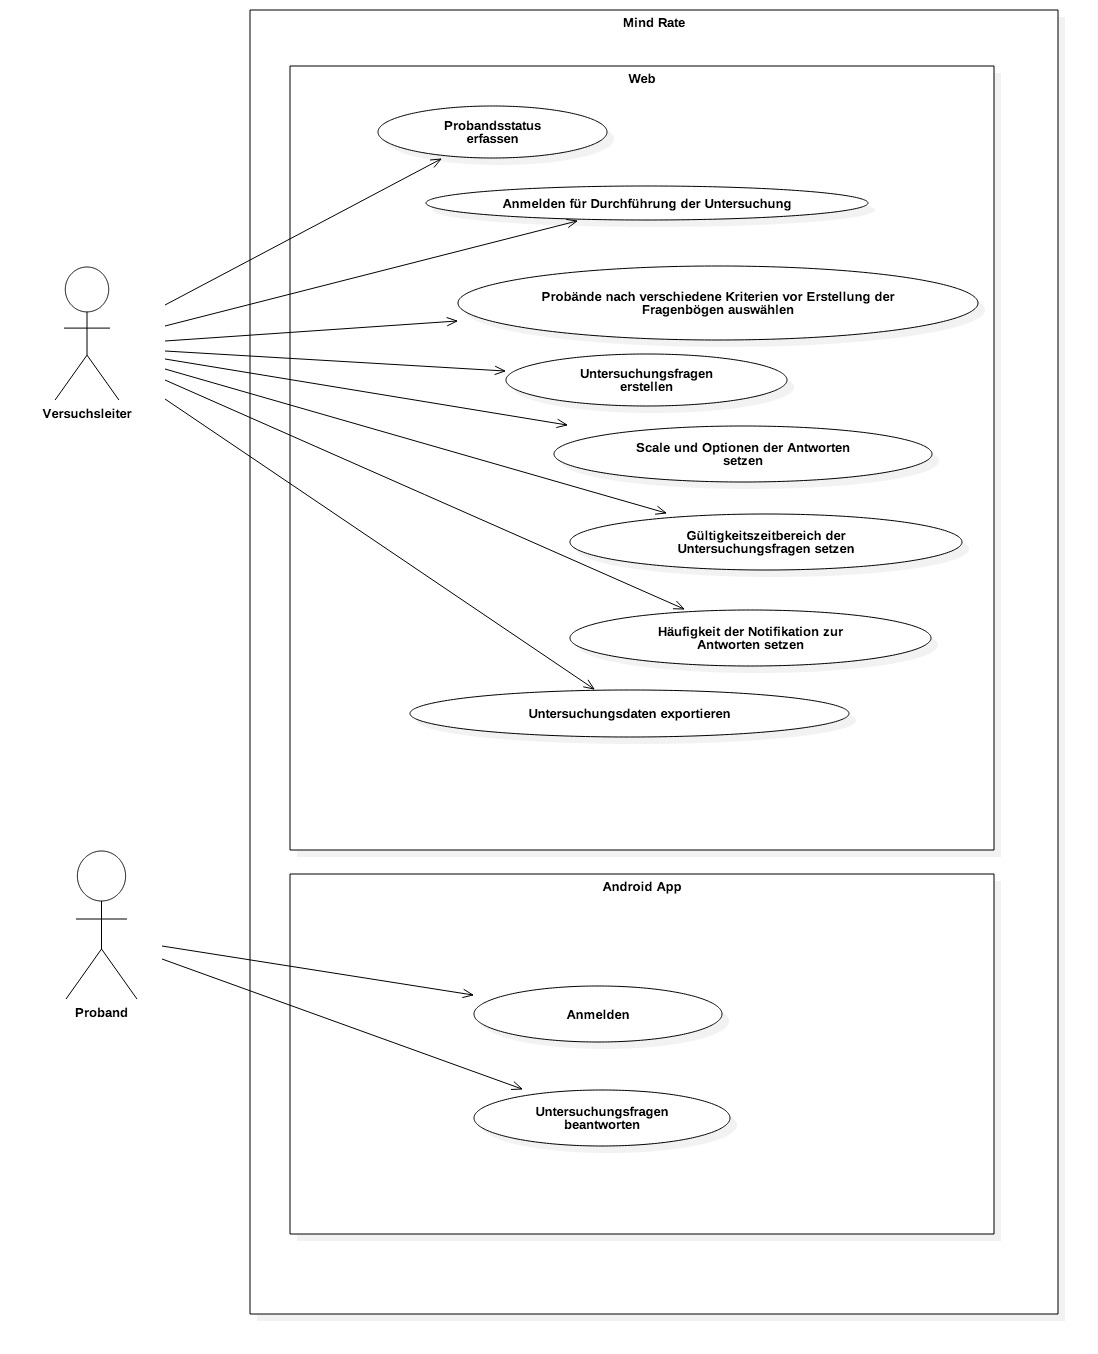
\includegraphics[scale = 0.4]{UseCaseDiagram1.jpg}
                \end{center}

        \newpage
        \section{Benutzerschnittstelle}
 
    \chapter{Qualitätsziele}
        Qualiätsziele: Allgemeine Ziele sind meistens Änderbarkeit und Wartbarkeit.
        Ziele sollten jedoch grundsätzlich messbar, spezifisch und relevant sein.
 
    \chapter{Glossar}
 
    % Abbildungsverzeichnis
    \listoffigures
 
\end{document}
